%% eval.tex
\chapter{Use-Case - Die Suche nach dem besten Auto}
\label{ch:useCase}
%% ==============================
Jeder hat beim Kauf eines Autos seine eigene Wünsche bzw. Kriterien. Beispielsweise wollen vielleicht viele eine hohe PS-Leistung, dafür interessiert andere nur ein günstiger Preis. Bei einem einzigen Kriterium, beispielsweise dass der Preis unter 16000 \euro{} liegen soll, kann es passieren, dass es zu viele Autos gibt, die dieses Kriterium erfüllen. Aus diesem Grund werden zuerst die Kundenwünsche in Präferenzen umgewandelt.
%% ==============================
\section{Datenvorbereitung}
\label{ch:Evaluierung:sec:vorbereitung}
%% ==============================
Zunächst werden jedoch alle Dimensionen der vorliegenden Datensätze beziehungsweise Autos vorgestellt. Die Dimensionen entsprechen den Spaltennamen der Autodaten und sind wie folgt benannt: id, name, make, color, price, age, horsepower, fuel, idowner, city\textunderscore consumption, mileage, description, reg\textunderscore date, highway\textunderscore consumption.

Die Daten liegen in einer PostgreSQL Datenbank vor. Mittels des Database Connector wird eine Verbindung zu dieser Datenbank hergestellt. Damit eine erfolgreiche Datenbankverbindung aufgebaut werden kann, müssen im NodeDialog dieses Nodes wichtige Daten wie Datenbank URL, JDBC Treiber, Username und Passwort eingegeben werden ({siehe Abbildung \ref{img:nodeDialogConnector}).

\begin{figure}[H]
	\centering
	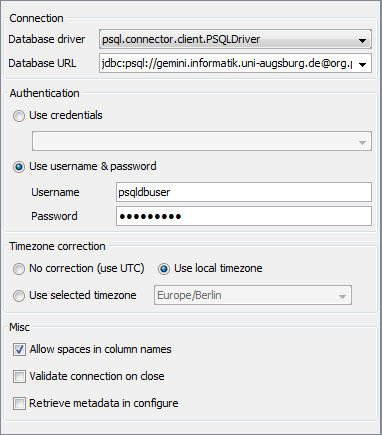
\includegraphics{nodeDialogConnector.png}
	\caption{NodeDialog des Database Connector Nodes}
	\label{img:nodeDialogConnector}
\end{figure} 

Der Node gibt eine Datenbankverbindung als Ausgabe zurück, die als Eingabe für den Database Table Selector und dem Database Reader Node dient. Diese beiden Nodes benötigen im NodeDialog einen SQL Query. Für dieses Beispiel wird der Query \textit{SELECT * FROM car} eingegeben, da mit allen Autodatensätzen und allen Dimensionen weitergearbeitet werden soll. Es ist jedoch möglich die Datensätze hier schon mit einer \textit{WHERE} Klausel einzuschränken.

Die Ausgabe des Database Table Selector ist die Datenbankverbindung, die als Eingabe in den Node kommt und mit dem eingegebenen Query als Zusatzinformation zurückgegeben wird. Der Database Reader gibt im Gegensatz dazu einen BufferedDataTable aus. Dieser entsteht durch die Abfrage des eingegebenen SQL Query an die Datenbank und stellt die Daten aller Autos mit ihren Dimensionen in einer Tabelle dar. 

Hierbei muss beachtet werden, dass beide Nodes eine identische Datenbankverbindung und den selben Query im NodeDialog als Eingabe bekommen sollten. Falls dies nicht der Fall ist, liefert der Preference Creator Node, der sowohl die Datenbankverbindung mit dem Query als auch den BufferedDataTable als Eingabe bekommt, einen Fehler.

Nachdem alle Vorbereitungen getroffen sind, können Präferenzen für die Wünsche der Kunden erstellt werden. Der bisherige Stand des KNIME Workflows ist in Abbildung \ref{img:datenVorbereitung} zu sehen.

\begin{figure}[H]
	\centering
	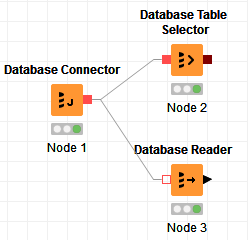
\includegraphics{datenVorbereitung.png}
	\caption{Workflow mit Database Connector, Database Table Selector und Database Reader Node}
	\label{img:datenVorbereitung}
\end{figure} 
%% ==============================
\section{Erstellung von Präferenzen}
\label{ch:Evaluierung:sec:createPref}
%% ==============================
Da nun die nötigen Eingaben für den Preference Creator vorhanden sind, können die Präferenzen für ausgewählte Dimensionen erstellt werden. Den BufferedDataTable benutzt dieser Node, um eine Auswahlbox für die Dimensionen und eine Auswahlbox für die Werte dieser Dimensionen zu erstellen. Die Datenbankverbindung wird für folgende Nodes benötigt, da diese mit den Score Query eine Scoretabelle erstellen können und mit diesen Scores anstatt der eigentlichen Daten weiterarbeiten. 
Der für dieses Kapitel ausgedachte Kunde hat folgende Präferenzen: Er möchte ein Auto mit einem niedrigen Preis, einer hohen PS-Leistung und einem niedrigen Kilometerstand. Darüber hinaus möchte er, dass das Auto nicht zu alt ist, was jedoch nicht so wichtig ist wie der Preis. Ebenfalls würde er ein grünes einem schwarzen Auto vorziehen und auf keinen Fall ein rotes Auto wollen. Wobei die Farbe nicht so wichtig wie die PS-Leistung ist.  Für die Farbe wird eine LAYERED Präferenz erstellt, was impliziert das dadurch der LayeredDialog geöffnet und die Farben entsprechend sortiert werden müssen. Für dieses Beispiel wird 'green' Layer 1, 'black' Layer 2 und 'red' Layer -1 hinzugefügt. Die restlichen Farben bleiben bei Layer 0 und sind somit indifferent.

Aus diesen Einstellungen ergeben sich die Präferenzen in Abbildung \ref{img:useCaseNodeDialog}. 

\begin{figure}[H]
	\centering
	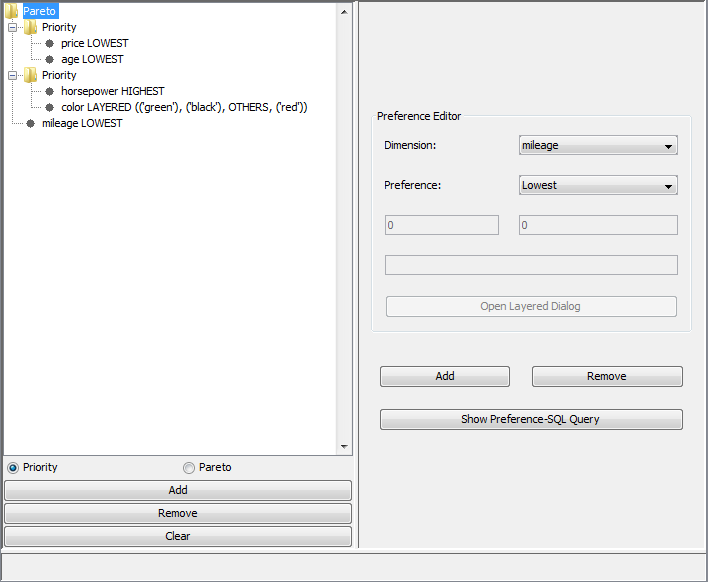
\includegraphics[width=\textwidth]{useCaseNodeDialog.png}
	\caption{Präferenzen für die Suche des besten Autos}
	\label{img:useCaseNodeDialog}
\end{figure} 

Nach der Ausführung des Nodes stehen die nötigen Daten (siehe Abbildung \ref{img:preferenceWorkflow}) für die (repräsentativen) Skyline Nodes wie den Distance Based Resolver zur Verfügung. 

\begin{figure}[H]
	\centering
	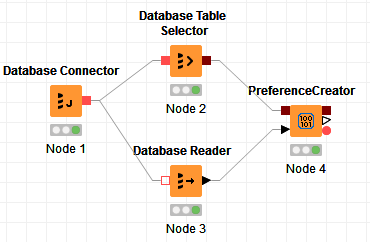
\includegraphics{preferenceWorkflow.png}
	\caption{Workflow mit dem Preference Creator Node}
	\label{img:preferenceWorkflow}
\end{figure}  
%% ==============================
\section{Reduzierung der Datensätze}
\label{ch:Evaluierung:sec:repSkyline}
%% ==============================
Wie erwähnt gibt der Preference Creator Node als Ausgabe eine Datenbankverbindung zurück. Mit dieser Verbindung kommen noch versteckte Flowvariablen in die nachfolgenden Nodes. Diese beinhalten Score Query, Preference Query und die formatierte Baumstruktur des NodeDialogs. Diese Datenbankverbindung und die Flowvariablen benutzt der Block Nested Loop Node, um eine Skyline zu erstellen. Im NodeDialog des Block Nested Loop Nodes, wurde für das Fenster des Algorithmus ein Wert von vier eingegeben, da dieser Wert für die 300 Datensätze  nicht zu groß und nicht zu klein ist. Nach Ausführung des Nodes wird eine Skyline mit 27 Datensätzen ausgegeben, die in Abbildung \ref{img:skyline} zu sehen ist. Es sind nur noch die Datensätze vorhanden, die basierend auf den Präferenzen  beziehungsweise den Scores nicht schlechter sind als andere.

\begin{figure}[H]
	\centering
	
\includegraphics[width=\textwidth]{skyline.png}
	\caption{Skyline des Autobeispiels}
	\label{img:skyline}
\end{figure} 

Mit dieser Anzahl von Skylinedatensätzen ist es jedoch immer noch schwer das beste Auto für den Kunden auszuwählen. Aus diesem Grund muss ergänzend die repräsentative Skyline bestimmt werden.

Der Diversity Significance Based Resolver beachtet sowohl Signifikanz als auch Diversität. Um signifikante Datensätze zu bestimmen, müssen die bereits existierenden Präferenzen mit weiteren Präferenzen erweitert werden. Für dieses Beispiel entscheidet der Kunde, dass er kein Auto mit einem höheren Preis als 16000 \euro{} haben möchte. Ergänzend sollte das Auto mehr als 100 PS besitzen. Somit wird für die Dimension price eingestellt, dass ein einzelner Threshold als obere Grenze berücksichtigt werden soll. Für die Dimension horsepower wird auch ein einzelner Threshold benutzt, jedoch als untere Grenze. Somit sind Autos signifikant, falls der Preis kleiner oder gleich 16000 \euro{} ist und die PS-Leistung 100 oder mehr beträgt.
Für dieses Beispiel wird angenommen, dass Signifikanz wichtiger ist als Diversität. Aus diesem Grund wird der Diversitätsfaktor gleich $0.4$ gesetzt und dadurch wird der Signifikanzfaktor automatisch auf $0.6$ gesetzt. Für $k$ wird wieder ein Wert von vier eingestellt, da aus dieser kleinen Menge ein passendes Auto für den Kunden herausgesucht werden kann und nicht zu viele durch den Algorithmus wegfallen. Das Ergebnis dieses Algorithmus kann in Figur \ref{img:eGreedyOutput} betrachtet werden.

\begin{figure}[H]
	\centering
	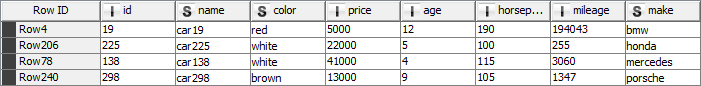
\includegraphics[width=\textwidth]{eGreedyOutput.png}
	\caption{Repräsentative Skyline des Diversity Significance Based Resolver}
	\label{img:eGreedyOutput}
\end{figure} 

Der Distance Based Resolver kann nur die Scores der ersten zwei Präferenzen bei der Bestimmung der repräsentativen Skyline berücksichtigen. Aus Demonstrationsgründen wurde der Node trotzdem mit den vorhandenen Präferenzen ausgeführt. Das Ergebnis des Nodes ist in Abbildung  \ref{img:distanceOutput} zu erkennen.

\begin{figure}[H]
	\centering
	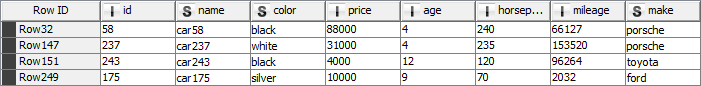
\includegraphics[width=\textwidth]{distanceOutput.png}
	\caption{Repräsentative Skyline des Distance Based Resolver}
	\label{img:distanceOutput}
\end{figure} 

Als letztes wird der Domination Maximizer benutzt, um die repräsentative Skyline zu bestimmen. Für diesen Node muss im NodeDialog die Größe der repräsentativen Skyline eingegeben werden. Für  das Beispiel dieses Kapitels, wurde der Wert $k=4$ genommen. Es ergibt sich die repräsentative Skyline in Abbildung \ref{img:domMaximizerOutput}. 

An den repräsentativen Skylines der anderen Nodes ist zu erkennen, dass die ausgegebenen Datensätze des Domination Maximizer bezüglich der numerischen Werte 'price', 'horsepower' und 'age' nah aneinander liegen. Das erklärt sich dadurch, dass der Algorithmus die Datensätze sucht, sodass die Anzahl der dominierten Datensätze maximal ist.

\begin{figure}[H]
	\centering
	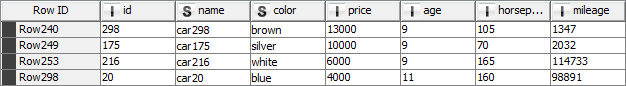
\includegraphics[width=\textwidth]{domMaximizerOutput.png}
	\caption{Repräsentative Skyline des Domination Maximizer}
	\label{img:domMaximizerOutput}
\end{figure} 

Der aktuelle Workflow, mit allen repräsentativen Skyline Nodes und dem zusätzlichen Block Nested Loop Node, kann in Abbildung \ref{img:skylineWorkflow} gesehen werden.

\begin{figure}[H]
	\centering
	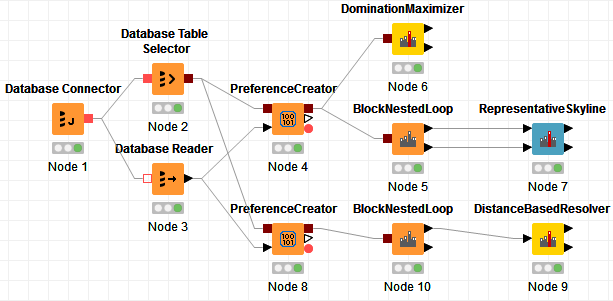
\includegraphics[width=\textwidth]{skylineWorkflow.png}
	\caption{Workflow mit Block Nested Loop, Diversity Significance Based Resolver und Distance Based Resolver Nodes}
	\label{img:skylineWorkflow}
\end{figure} 
%% ==============================
\section{Visualisierung}
\label{ch:Evaluierung:sec:visualize}
%% ==============================
Für die Visualisierung der Ausgaben der Nodes wird der (Representative) Skyline Visualizer verwendet. Dieser bekommt als Eingabe zwei BufferedDataTables und erstellt mit diesen Daten ein Koordinatensystem mit dominierten und undominierten Punkten.  

Die Ausgaben des Diversity Significance Based Resolver, Domination Maximizer und des Distance Based Resolver Nodes sind repräsentative Skylines. Für eine repräsentative Skyline besteht das Koordinatensystem aus den repräsentativen Skylinepunkten als undominierte Punkte und den Skylinepunkten als dominierte Punkte. Falls drei Dimensionen betrachtet werden, erstellt der (Representative) Skyline Visualizer für jede Kombination der Dimensionen einen Graphen. Aus diesem Grund werden bei mehr als drei Dimensionen keine Graphen mehr erstellt. Jedoch können im NodeDialog die Dimensionen ausgewählt werden die im View angezeigt werden sollen. Infolgedessen wird für das Beispiel dieses Kapitels die Visualisierung auf die Dimensionen 'price' und 'horsepower' reduziert.

Der Graph des Diversity Significance Based Resolver Nodes kann in Abbildung \ref{img:eGreedyView} gesehen werden. Wohingegen die Graphen des Distance Based Resolver in Abbildung \ref{img:distBasedResolverView} und des Domination Maximizer in Abbildung \ref{img:domMaximizerView} betrachtet werden können. 
	
	\begin{figure}[H]
	\centering
	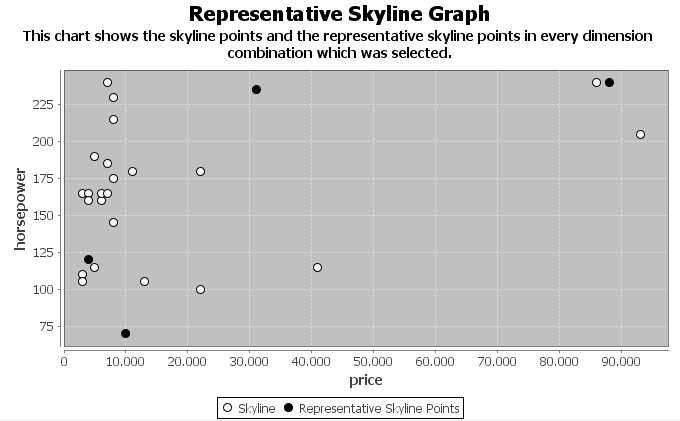
\includegraphics[width=\textwidth]{eGreedyView.png}
	\caption{(Representative) Skyline Visualizer View für die Ausgabe des Diversity Significance Based Resolver Nodes}
	\label{img:eGreedyView}
\end{figure} 

\begin{figure}[H]
	\centering
	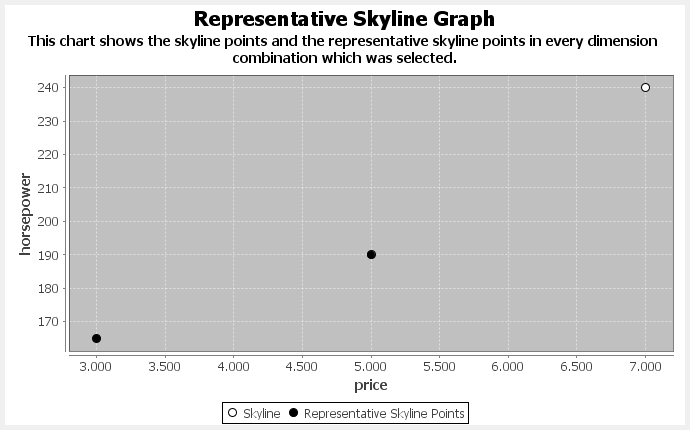
\includegraphics[width=\textwidth]{distBasedResolverView.png}
	\caption{(Representative) Skyline Visualizer View für die Ausgabe des Distance Based Resolver Nodes}
	\label{img:distBasedResolverView}
\end{figure} 

\begin{figure}[H]
	\centering
	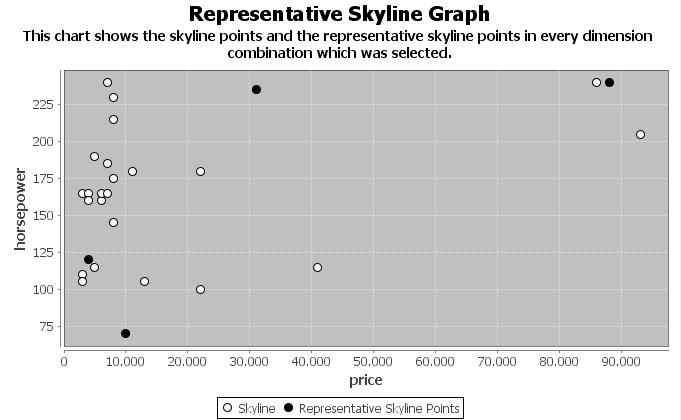
\includegraphics[width=\textwidth]{domMaximizerView.png}
	\caption{(Representative) Skyline Visualizer View für die Ausgabe des Domination Maximizer Nodes}
	\label{img:domMaximizerView}
\end{figure} 

Der derzeitige Workflow mit den zusätzlichen Visualizer Nodes wird in Abbildung \ref{img:visualizeWorkflow} dargestellt.

\begin{figure}[H]
	\centering
	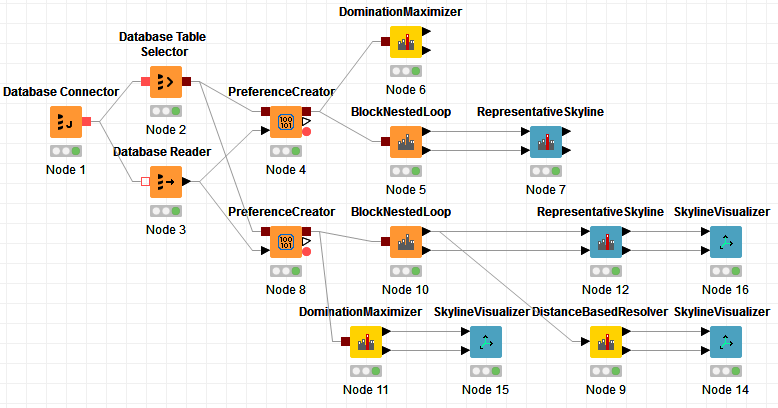
\includegraphics[width=\textwidth]{visualizeWorkflow.png}
	\caption{Workflow mit den (Representative) Skyline Visualizer Nodes}
	\label{img:visualizeWorkflow}
\end{figure} 

%% ==============================
\section{Preference-SQL}
\label{ch:Evaluierung:sec:prefSQL}
%% ==============================
Schlussendlich werden der Preference SQL Extract und der Preference SQL Node zum Workflow hinzugefügt. Mithilfe des Preference SQL Extract Nodes wird der Preference Query ausgegeben und kann in einem BufferedDataTable betrachtet und kopiert werden. Diesen Query benutzt der Preference SQL Node hingegen, um mittels des Best Matches Models die besten Datensätze basierend auf den Präferenzen auszugeben.

Der Preference Query für die in diesem Kapitel erstellten Präferenzen lautet:
 
\begin{verbatim}
SELECT * 
FROM (SELECT * FROM car) AS T 
PREFERRING ((price LOWEST PRIOR TO age LOWEST) 
AND (horsepower HIGHEST 
PRIOR TO color LAYERED (('green', 'black'), OTHERS, ('red')))
AND mileage LOWEST)
\end{verbatim}

Nach Hinzufügen des Preference SQL Extract und des Preference SQL Nodes, ist der vollständige Workflow in Abbildung \ref{img:finalWorkflow} zu sehen. 
 
\begin{figure}[H]
	\centering
	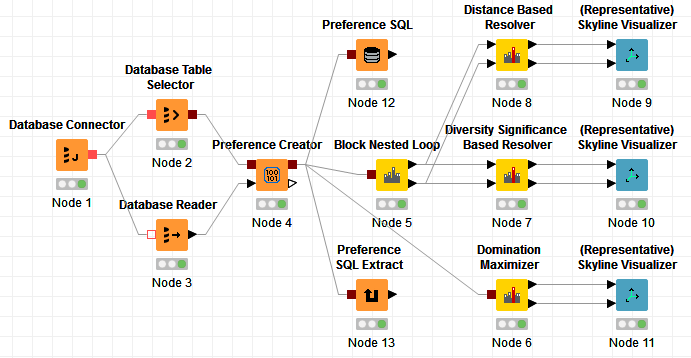
\includegraphics[width=\textwidth]{finalWorkflow.png}
	\caption{Workflow mit Preference SQL Extract und Preference SQL Node}
	\label{img:finalWorkflow}
\end{figure} 
%% ==============================
\section{Evaluierung der implementierten KNIME Nodes}
\label{ch:Evaluierung:sec:zusammenfassung}
%% ==============================
Die Datensätze der repräsentativen Skyline können dem Kunden zum Schluss vorgezeigt werden. Woraufhin dieser sich für eines der Autos entscheiden kann. Es ist zu erkennen, dass der Kunde mit vier Autos eine übersichtlichere Menge für die Entscheidung hat als bei 27 vorliegenden Datensätzen.

Zusammenfassend kann gesagt werden, dass die KNIME Nodes intuitiv und einfach nutzbar sind. Durch die Auswahl und Eingrenzen der Kriterien mithilfe der Nodes konnten schnell die besten Auto für die Präferenzen des Kunden gefunden werden. Visualisierungen helfen dabei die repräsentativen Datensätze einordnen zu können. 
%% ==============================
%%% End: 